\addcontentsline{toc}{chapter}{Appendix 5}\label{ch:Falcon9}
\chapter{Falcon 9 v1.1 flight performance}

In order to develop relevant solutions to  problems in industry, it is important to have an understanding of what the real world challenges faced by the receiver are. A thorough understanding of the real world challenges allows accurate simulations analysis to be carried out.

\begin{figure}[!htb] 
    \centering
    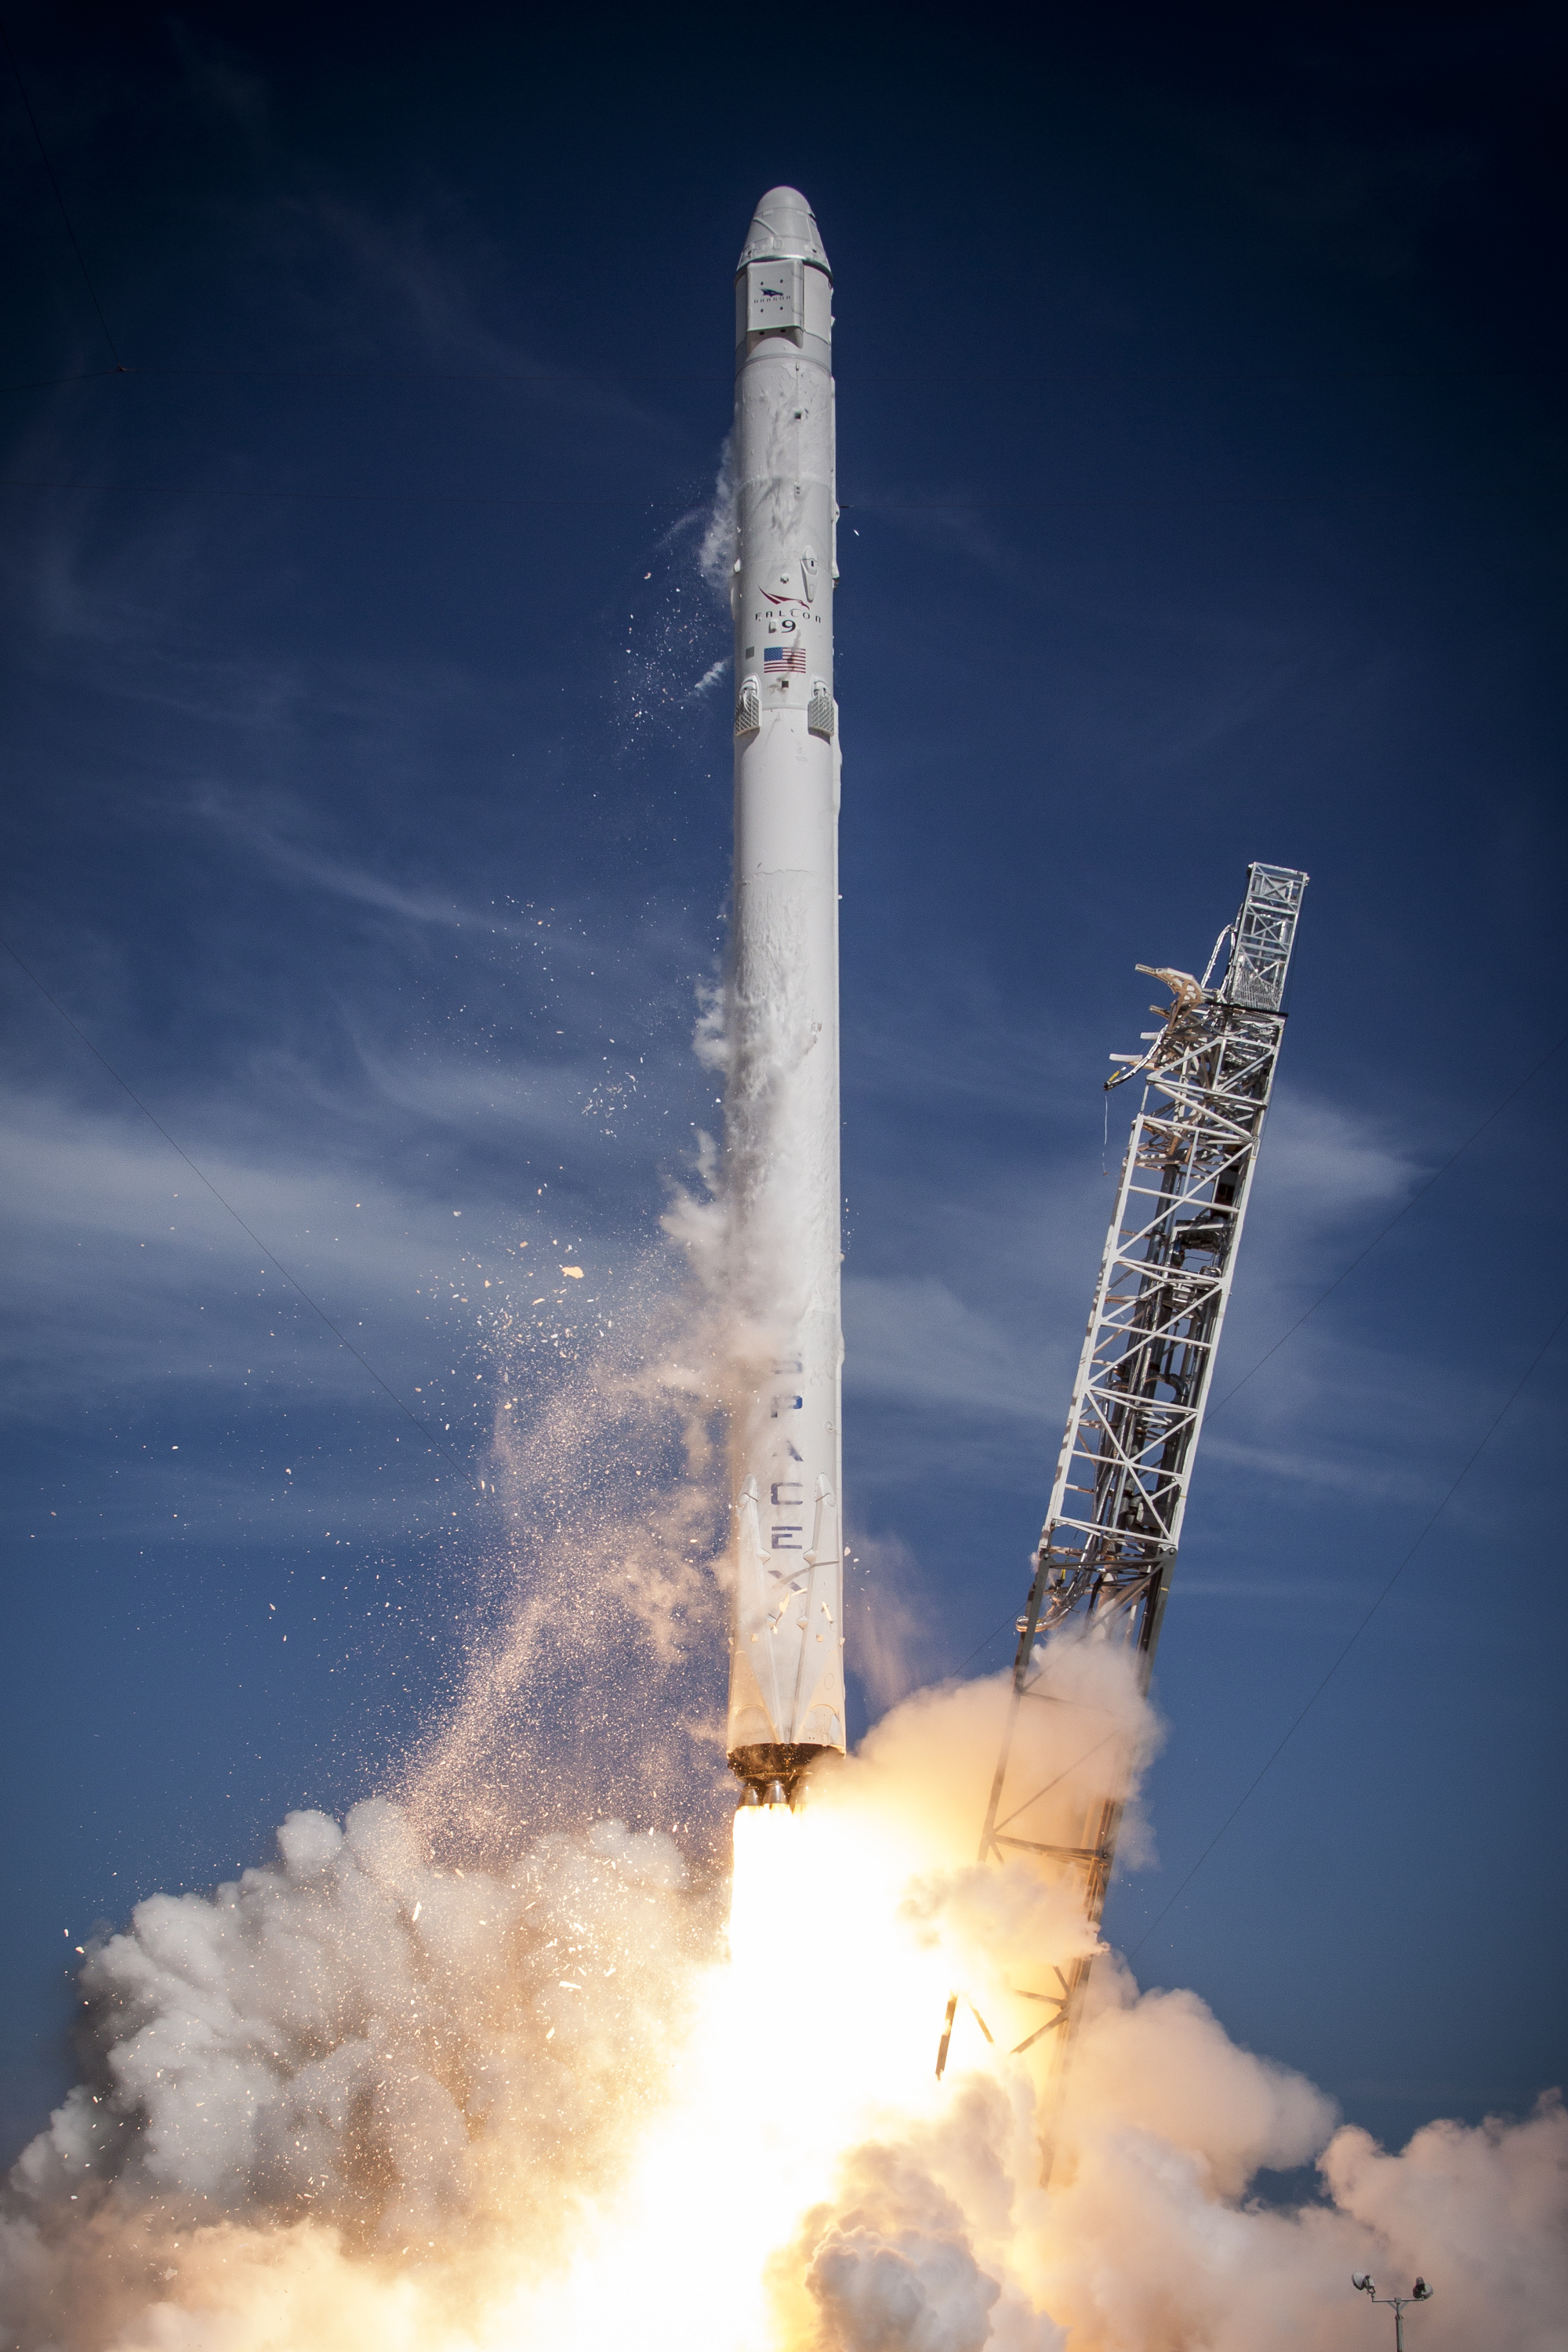
\includegraphics[width=0.9\textwidth]{Falcon9/crs6_launch_center.jpg} 
    \caption{CRS-6 Launch, Image from \cite{SpaceXPhotos}}
    \label{fig:Falcon9}
\end{figure}


In order to meet this goal, the Falcon 9 v1.1 was chosen for analysis. There were a number of reasons for this choice, in particular, the Falcon 9 is gaining industry acceptance, and is likely to represent a significant market share of launches going forward. Additionally, Space Exploration Technology Corporation (SpaceX) who develop,construct and launch the Falcon 9 are more open regarding the technical details of their \ac{LV} than their contemporaries. Finally, the Falcon 9 v1.1 is experiences a wide variety of dynamics, including the first stage conducting a "hover slam" or "suicide burn" manoeuvre, the success of which is reliant on accurate position and velocity estimates.

Because the actual flight performance of the Falcon 9 v1.1 is proprietary and confidential, an effort must be made to develop an model which uses publicly disclosed information. In this manner, a model of the performance can be developed, and compared against real world performance of the \ac{LV}.

\section{Physics model}

\begin{figure}[!htb] 
    \centering
    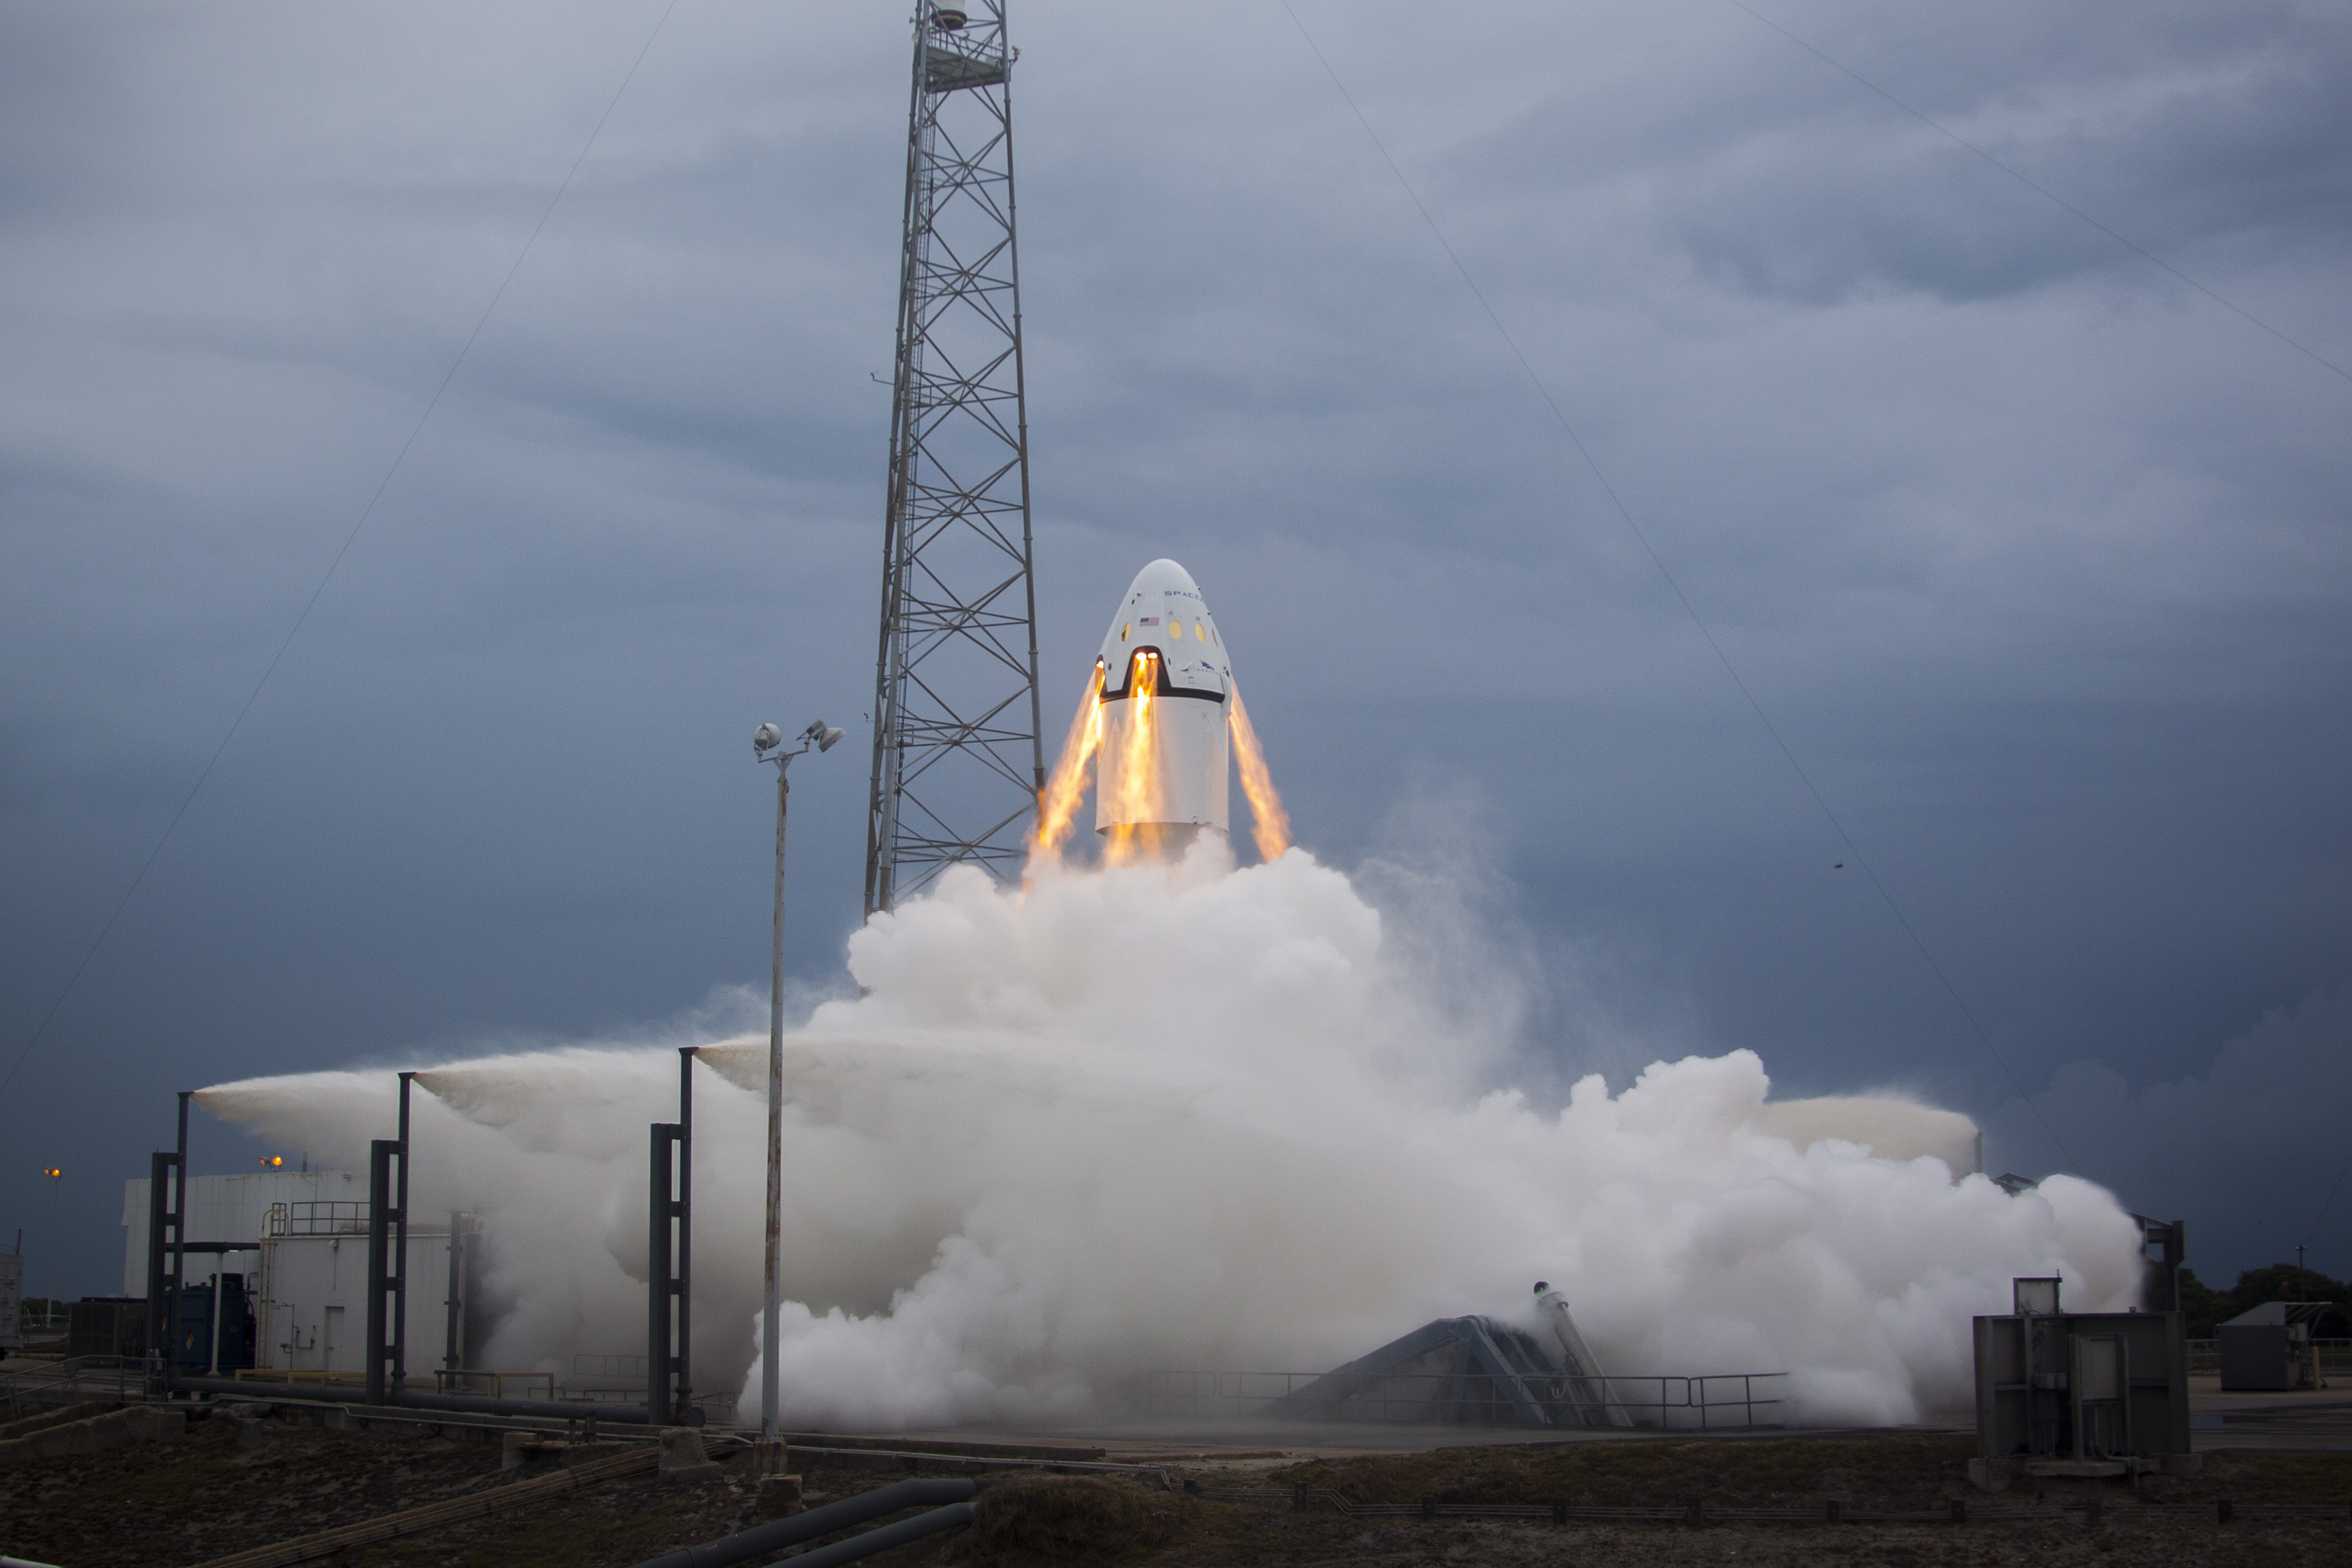
\includegraphics[width=0.9\textwidth]{Falcon9/dragon_pad_abort_launch2.jpg} 
    \caption{Pad abort testing, Image from \cite{SpaceXPhotos}}
    \label{fig:PadAbort}
\end{figure}

\section{Measured performance}

In order to verify the physics model, it must be compared against real world data. Because the true flight performance is proprietary and confidential, the publicly released videos and associated commentary of three different launches were transcribed. 

\begin{table}[!htb]
\centering
\begin{tabular}{|l|l|}
\hline
\rowcolor[HTML]{C0C0C0} 
Time (s) & Event                                \\ \hline
60       & 5.8km alt, 250m/s, 0.8km down range  \\ \hline
\rowcolor[HTML]{EFEFEF} 
86       & Max Q                                \\ \hline
127      & 38km alt, 1160m/s, 19km down range   \\ \hline
\rowcolor[HTML]{EFEFEF} 
150      & 61km alt, 1900m/s, 40km down range   \\ \hline
169      & Stage 1 separation                   \\ \hline
\rowcolor[HTML]{EFEFEF} 
180      & 93km alt, 2120m/s, 79km down range   \\ \hline
265      & 156km alt, 2500m/s, 193km down range \\ \hline
\rowcolor[HTML]{EFEFEF} 
380     & 202km alt, 3700m/s, 420km down range \\ \hline
454      & 210km alt, 4700m/s, 610km down range \\ \hline
\rowcolor[HTML]{EFEFEF} 
540      & 207km alt, 6700m/s, 925km down range \\ \hline
\end{tabular}
\caption{CRS-4 Flight transcript \cite{CRS4}}
\label{tab:CRS4}
\end{table}

\begin{table}[!htb]
\centering
\begin{tabular}{|l|l|}
\hline
\rowcolor[HTML]{C0C0C0} 
Time (s) & Event                                \\ \hline
60       & 5.5km alt, 250m/s 0.9km down range   \\ \hline
\rowcolor[HTML]{EFEFEF} 
97       & Max Q                                \\ \hline
126      & 35km alt, 1000m/s 14.5 km down range \\ \hline
\rowcolor[HTML]{EFEFEF} 
150      & 58km alt, 1800m/s 33 km down range   \\ \hline
165      & Stage 1 seperation                   \\ \hline
\rowcolor[HTML]{EFEFEF} 
185      & 90km alt, 1900m/s 67km down range    \\ \hline
240      & 134km alt, 2100m/s, 135km down range \\ \hline
\rowcolor[HTML]{EFEFEF} 
270      & Stage 1 boost-back start             \\ \hline
300      & 166km alt, 2600m/s                   \\ \hline
\rowcolor[HTML]{EFEFEF} 
316      & Stage 1 boost-back stop              \\ \hline
412      & Stage 1 entry burn start             \\ \hline
\rowcolor[HTML]{EFEFEF} 
428      & Stage 1 entry burn stop              \\ \hline
435      & 205km alt, 4200km, (garbled) down range    \\ \hline
\rowcolor[HTML]{EFEFEF} 
475      & Stage 1 transonic                    \\ \hline
514      & Stage 1 under horizon                \\ \hline
\rowcolor[HTML]{EFEFEF} 
540      & 208km, 6900m/s 850km down range      \\ \hline
565      & Stage 2 engine shutdown              \\ \hline
\end{tabular}
\caption{CRS-5 Flight transcript \cite{CRS5}}
\label{tab:CRS5}
\end{table}

\begin{table}[!htb]
\centering
\begin{tabular}{|l|l|}
\hline
\rowcolor[HTML]{C0C0C0} 
Time (s) & Event                                 \\ \hline
120      & 32km alt, 1000m/s, 13.5km down range  \\ \hline
\rowcolor[HTML]{EFEFEF} 
165      & Stage seperation                      \\ \hline
180      & 86km alt, 1950m/s, 63km down range    \\ \hline
\rowcolor[HTML]{EFEFEF} 
277      & Stage 1 boost-back start              \\ \hline
300      & 165km alt, 2560m/s, 212km down range  \\ \hline
\rowcolor[HTML]{EFEFEF} 
315      & Stage 1 boost-back stop               \\ \hline
405      & Stage 1 entry burn start              \\ \hline
\rowcolor[HTML]{EFEFEF} 
425      & Stage 1 entry burn stop               \\ \hline
450      & 205km alt, 4400m/s, 530km down range  \\ \hline
\rowcolor[HTML]{EFEFEF} 
491      & Stage 1 transonic                     \\ \hline
540      & 208 km alt, 6500m/s, 830km down range \\ \hline
\rowcolor[HTML]{EFEFEF} 
574      & Stage 2 shutdown \\ \hline
\end{tabular}
\caption{CRS-6 Flight transcript \cite{CRS6}}
\label{tab:CRS6}
\end{table}



\begin{figure}[!htb]
\centering

\includegraphics[scale=1]{Falcon9/Falcon9R.pdf}
\caption{Falcon 9 Rocket}
\label{fig:Rocket}
\end{figure}

\section{Velocity Requirements}
The 2nd stage burn must be terminated at precisely the right time, to ensure that the final velocity is correct. This is because the orbital height is dictated by the velocity, 

\begin{equation}
v_0 = \sqrt{\frac{G \cdot M}{r}}
\end{equation}

Where:
\begin{align*}
G &= 6.673 \times 10^{-11} N m^2 kg^{-2}\\
M &= 5.972 \times 10^{24} kg
\end{align*}

\begin{equation}
r = \frac{G \cdot M}{v_0^2}
\end{equation}

\begin{equation}
\frac{dr}{dv} = \frac{-2 \cdot G \cdot M}{v_0^3}
\end{equation}

For \ac{LEO}, with an orbital velocity of $\approx$ 7,800 m/s, this results in a a differential of 1,679m of altitude, per m/s of velocity. Given that SpaceX guarantees orbital height of $\pm$ 10km, this results in a velocity tolerance of $\pm$ 5.95 m/s, or $\pm$ 31.2 Hz of doppler shift.

\begin{table}[!htb]
\centering
\begin{tabular}{|l|l|l|l|l|l|}
\hline
\rowcolor[HTML]{C0C0C0} 
Date      & Vehicle       & No    & Payload      & Mass (Tons)         & Orbit                  \\ \hline
21/9/2014 & Falcon 9 v1.1 & F9-13 & CRS-4 Dragon & $\approx$ 9.3  & 199x359x51.64  LEO/ISS \\ \hline
\rowcolor[HTML]{EFEFEF} 
10/1/2015 & Falcon 9 v1.1 & F9-14 & CRS-5 Dragon & $\approx$ 9.54 & 206x353x51.6 LEO/ISS   \\ \hline
14/5/2015 & Falcon 9 v1.1 & F9-18 & CRS-6 Dragon & $\approx$ 9.24 & 199x364x51.65  LEO/ISS \\ \hline
\end{tabular}
\caption{My caption}
\label{FOOBAR}
\end{table}
\cite{Falcon9Stats}


\begin{table}[!htb]
\centering
\begin{tabular}{|l|l|}
\hline
\rowcolor[HTML]{C0C0C0} 
Time (s) & Event                                     \\ \hline
0.0      & Liftoff from Cape Canaveral               \\ \hline
\rowcolor[HTML]{EFEFEF} 
7.5      & Initial Pitch Kick                        \\ \hline
55.0     & Begin gravity turn                        \\ \hline
\rowcolor[HTML]{EFEFEF} 
76.0     & Max-Q                                     \\ \hline
115.0    & Release angle of attack restrictions      \\ \hline
\rowcolor[HTML]{EFEFEF} 
155.5    & Shutdown 2 engines for acceleration limit \\ \hline
174.2    & Main Engine Cut Off                       \\ \hline
\rowcolor[HTML]{EFEFEF} 
176.2    & Stage 1/Stage 2 separation                \\ \hline
179.2    & Second stage engine start \#1             \\ \hline
\rowcolor[HTML]{EFEFEF} 
199.2    & Payload fairing jettison                  \\ \hline
475.9    & Second stage engine cut off               \\ \hline
\end{tabular}
\caption{Falcon 9 Sample Flight Time-line \cite{Falcon9}}
\label{tab:Falcon9Timeline}
\end{table}

\begin{figure}[!htb] 
    \centering
    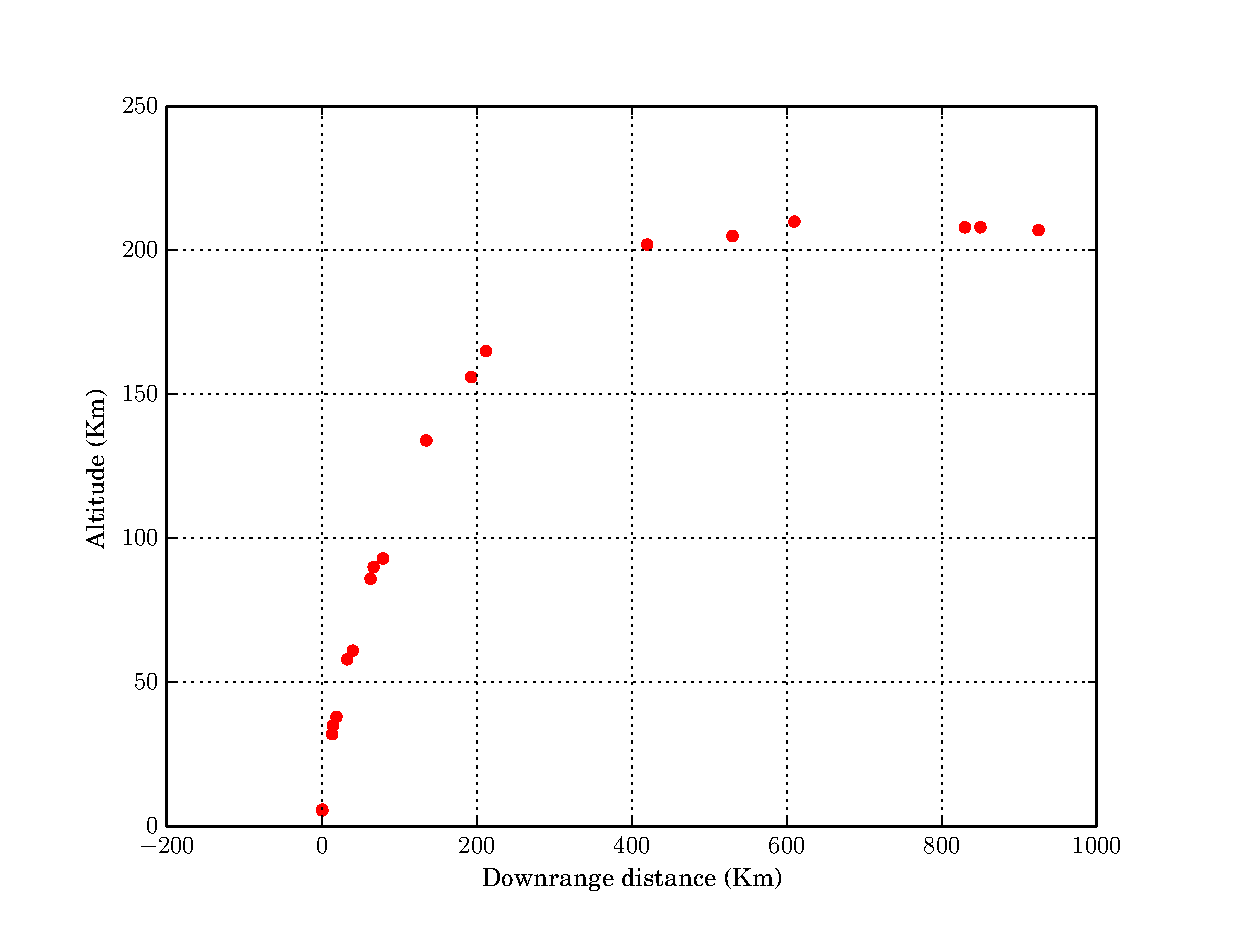
\includegraphics[width=1\textwidth]{Falcon9/FlightProfile.eps} 
    \caption{The Falcon 9 V1.1 flight profile, compare with figure \ref{fig:Falcon9Launch}.}
    \label{fig:Falcon9FlightProfile}
\end{figure}


\begin{figure}[!htb] 
    \centering
    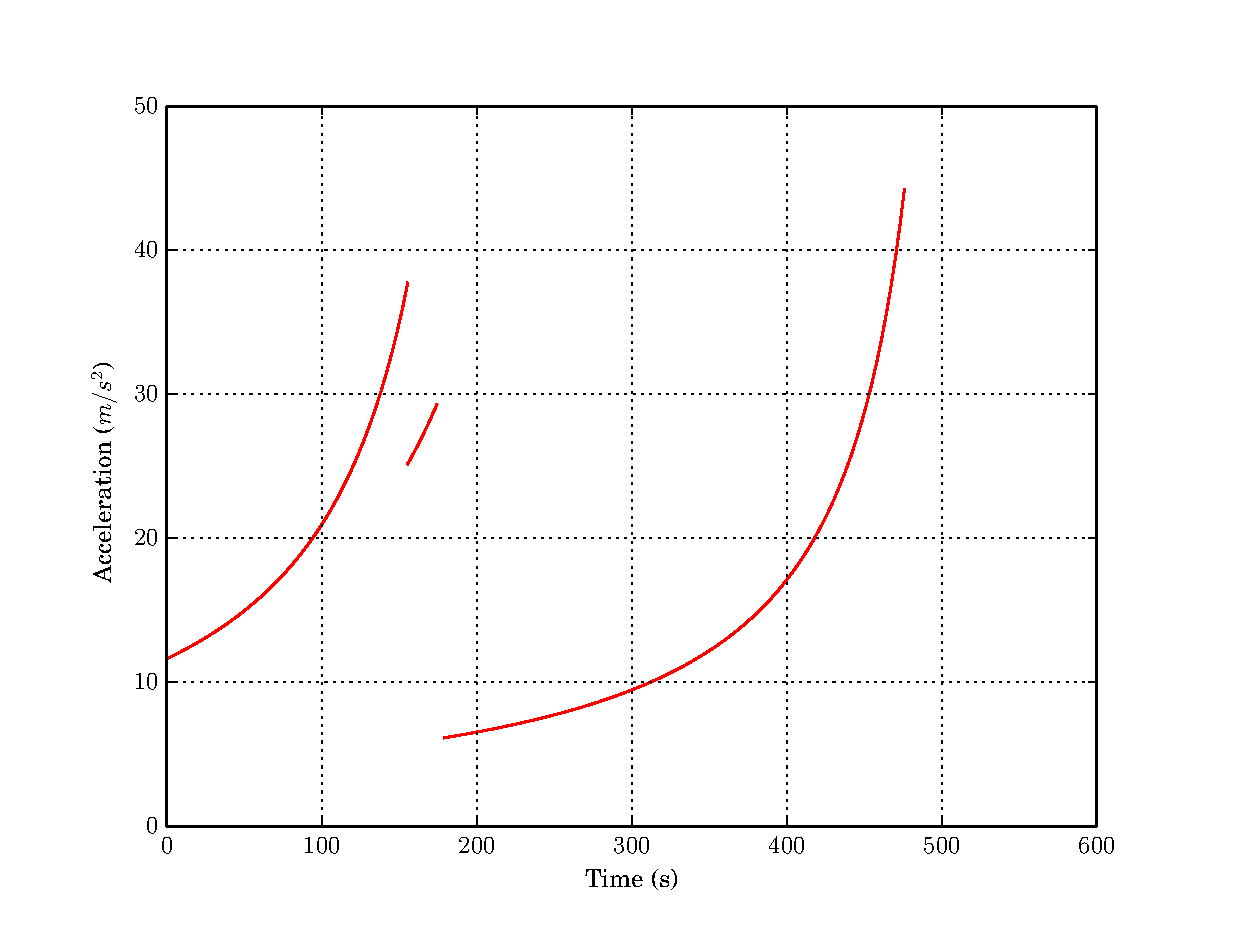
\includegraphics[width=1\textwidth]{Falcon9/Model.eps}
    \caption{}
    \label{fig:Falcon9Model}
\end{figure}


\begin{figure}[!htb] 
    \centering
    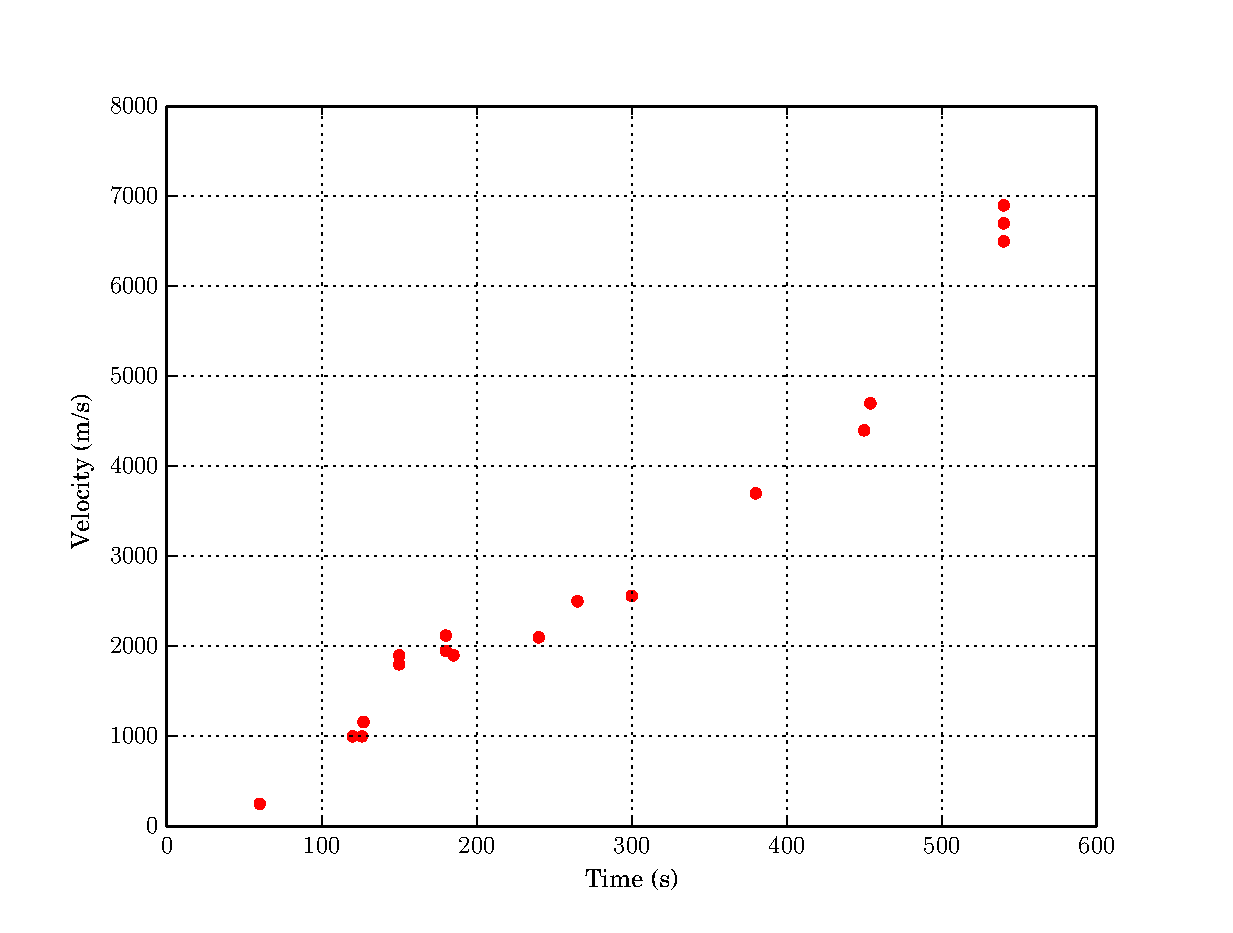
\includegraphics[width=1\textwidth]{Falcon9/VelocityProfile.eps}
    \caption{}
    \label{fig:Falcon9VelocityProfile}
\end{figure}



\begin{figure}[!htb] 
    \centering
    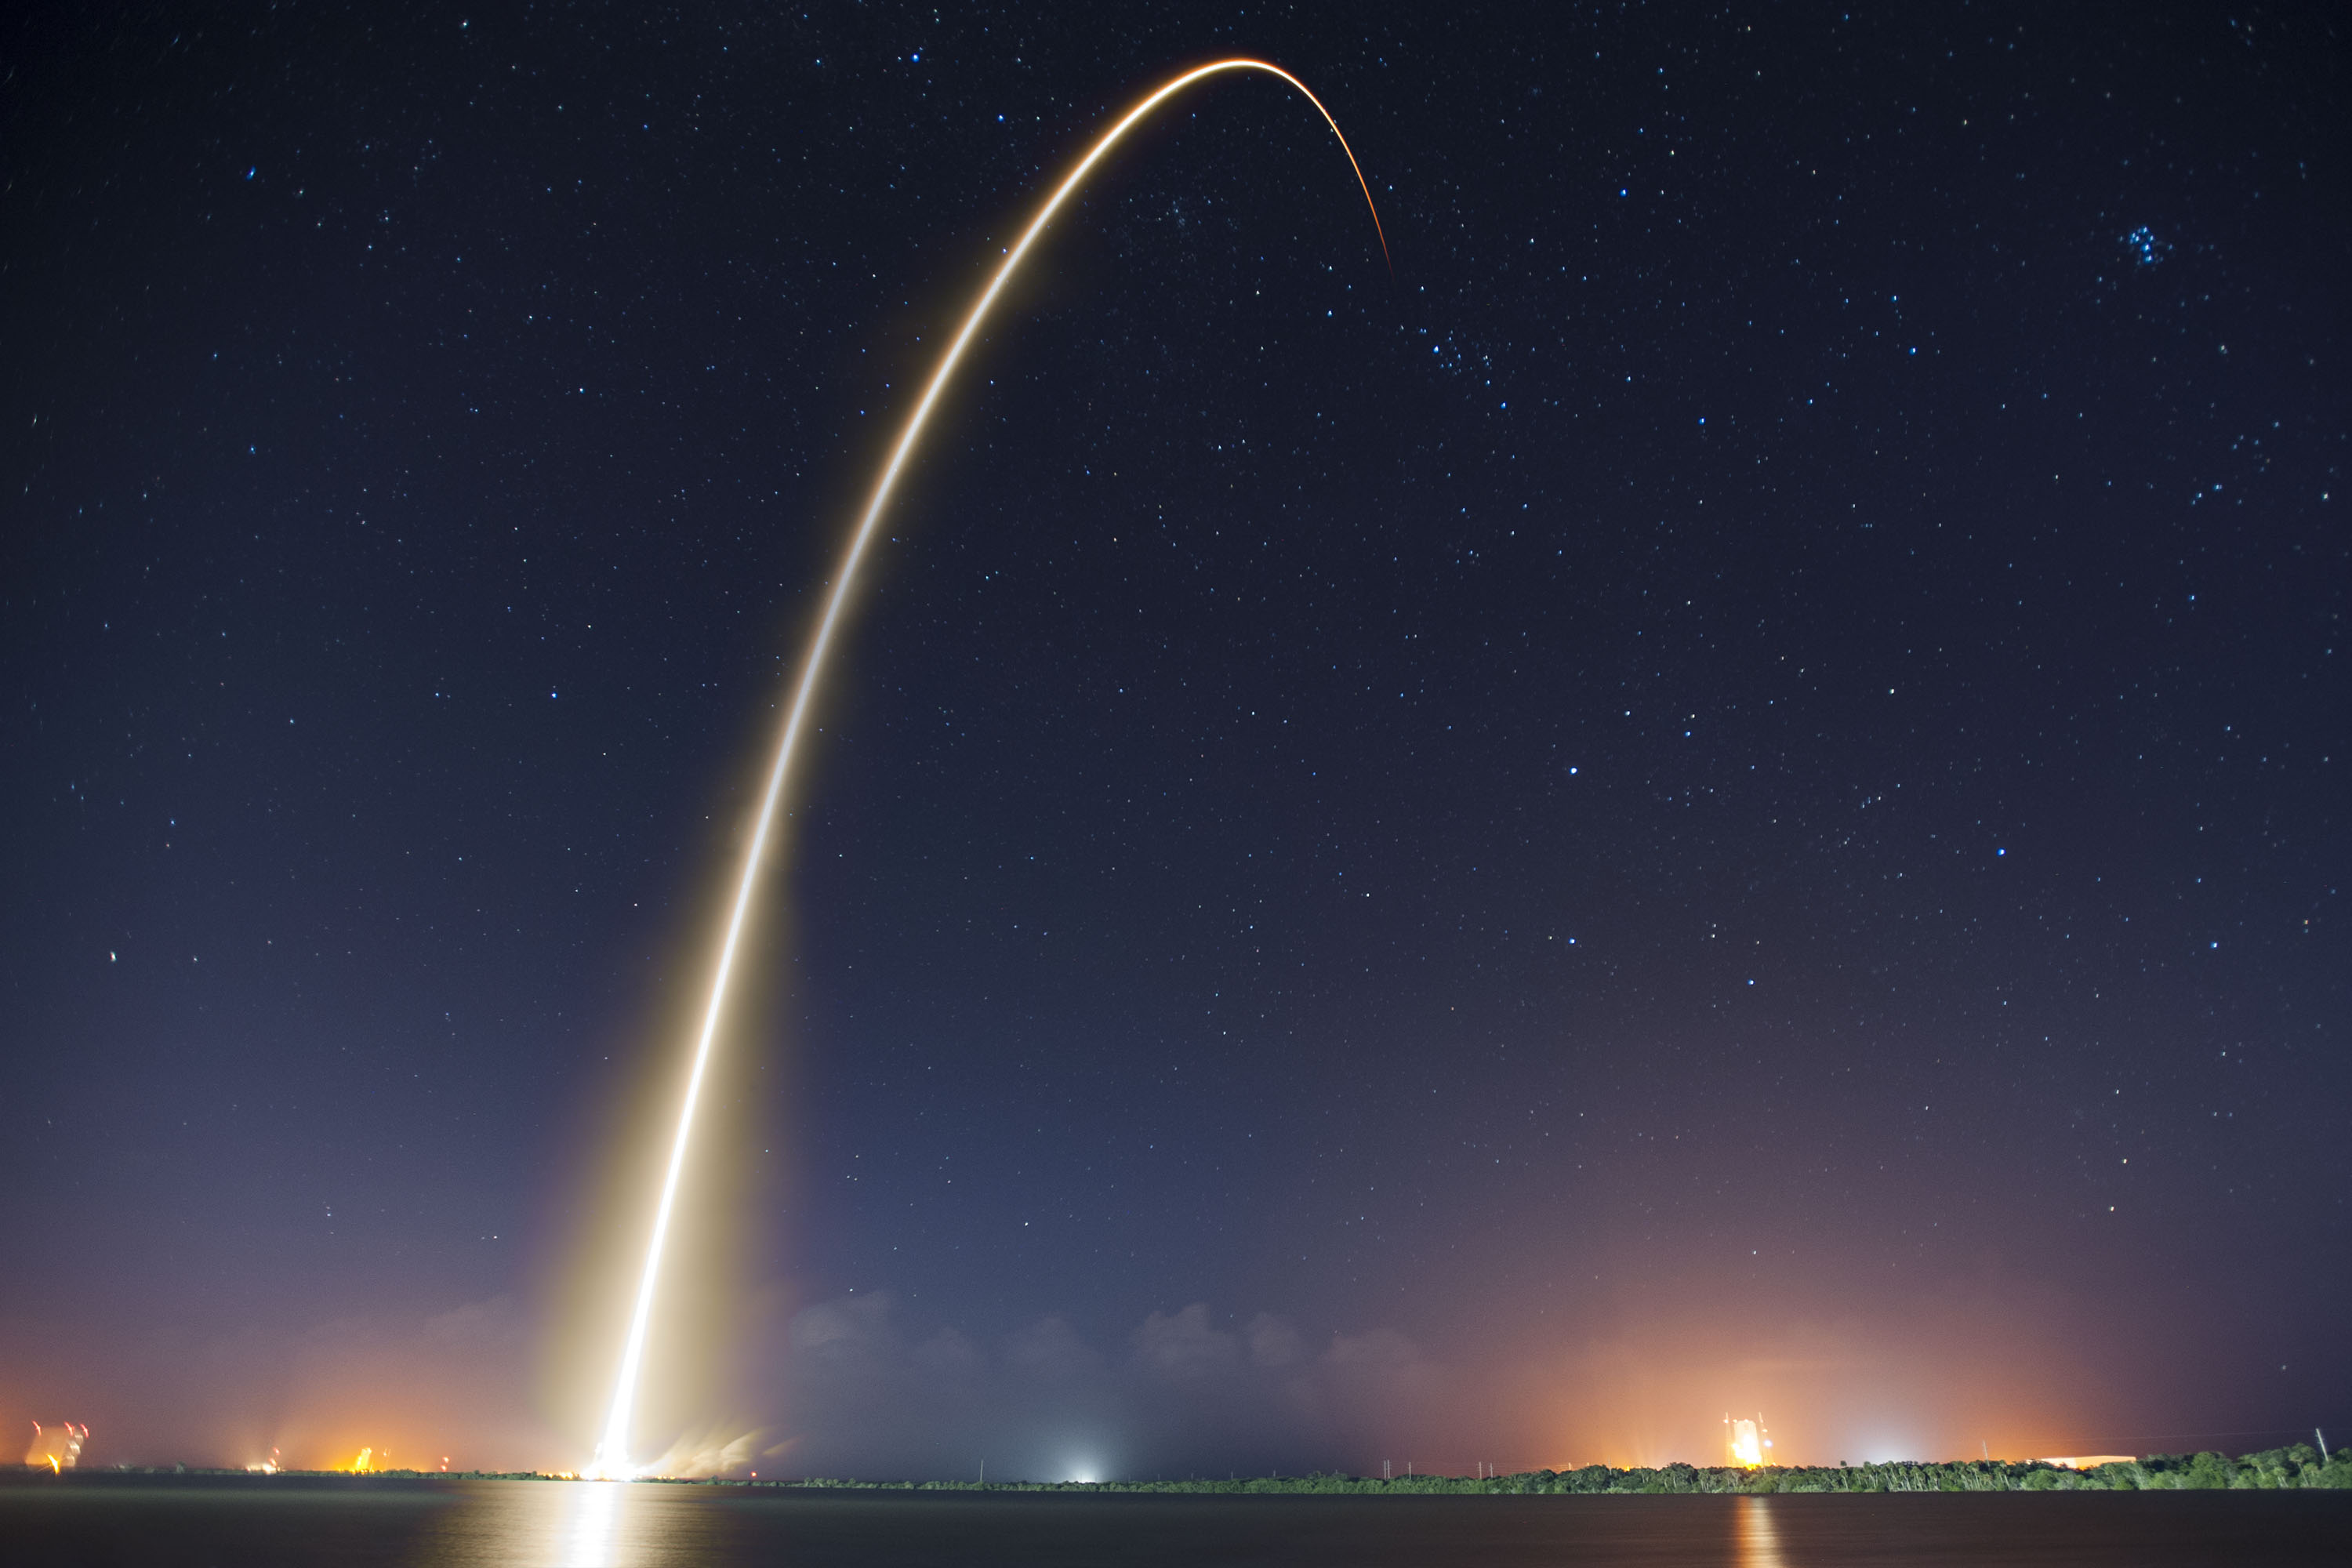
\includegraphics[width=1\textwidth]{Falcon9/Launch1.jpg}
    \caption{An oblique view of a Falcon 9 V1.1 launch. \cite{SpaceXFalcon9}}
    \label{fig:Falcon9Launch}
\end{figure}


\section{Launch Azimuth}

\begin{equation}
\beta = arcsin \Big(\frac{cos(i)}{cos(\phi)}\Big)
\end{equation}

Where:
\begin{align*}
 i &= \text{Orbit inclination}\\
 \phi &= \text{Launch site latitude}\\
 \beta &= \text{Launch azimuth}\\
\end{align*}

\cite{LaunchDesign}

The \ac{ISS} has an inclination of $51.6\degree$, hence a launch from Cape Canaveral ($\phi = 28.5\degree$), $\beta=44.9\degree$.


\begin{figure}[!htb] 
    \centering
    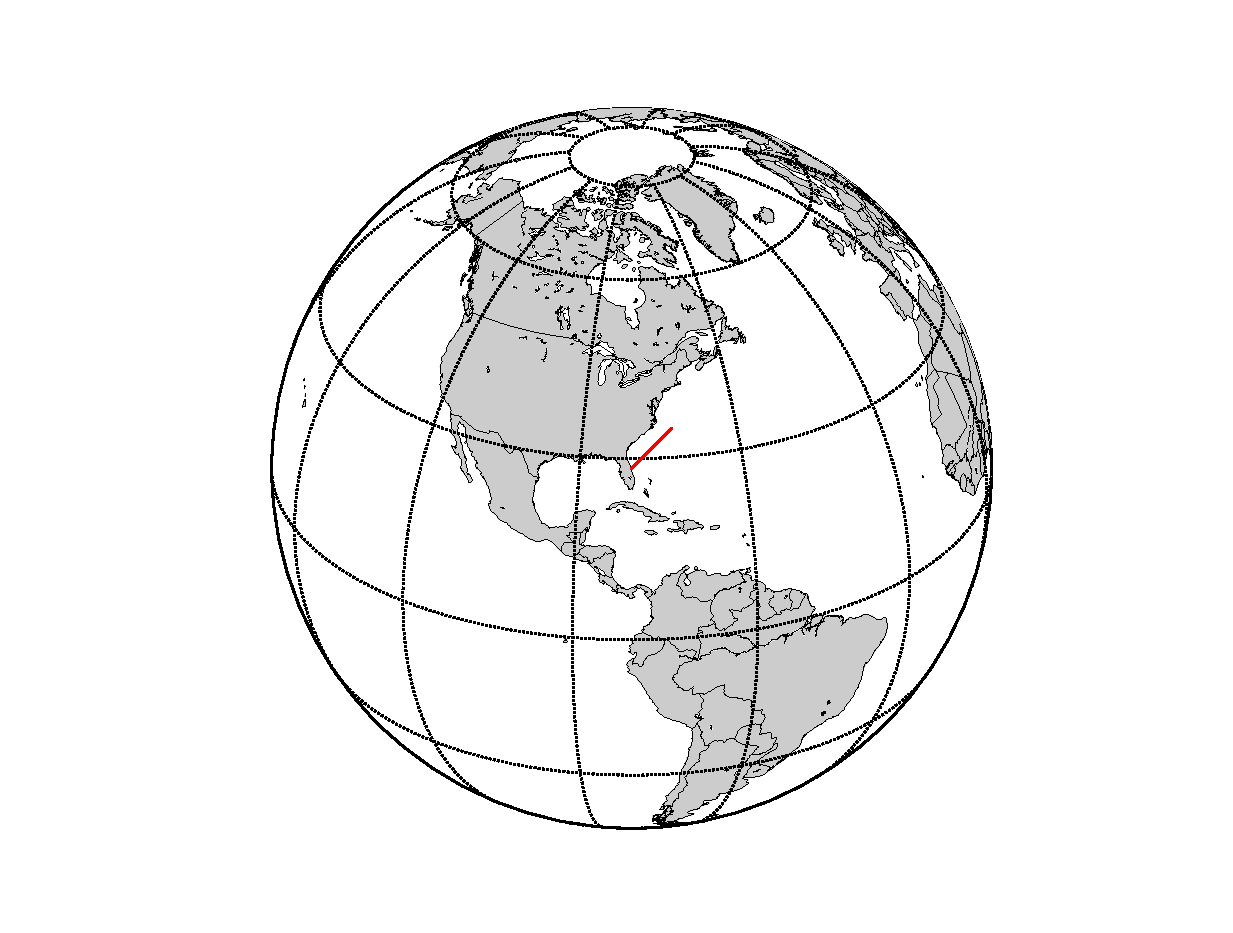
\includegraphics[width=1\textwidth]{Falcon9/CapeCanaveral.eps}
    \caption{}
    \label{fig:LaunchPath}
\end{figure}


\begin{figure}[!htb] 
    \centering
    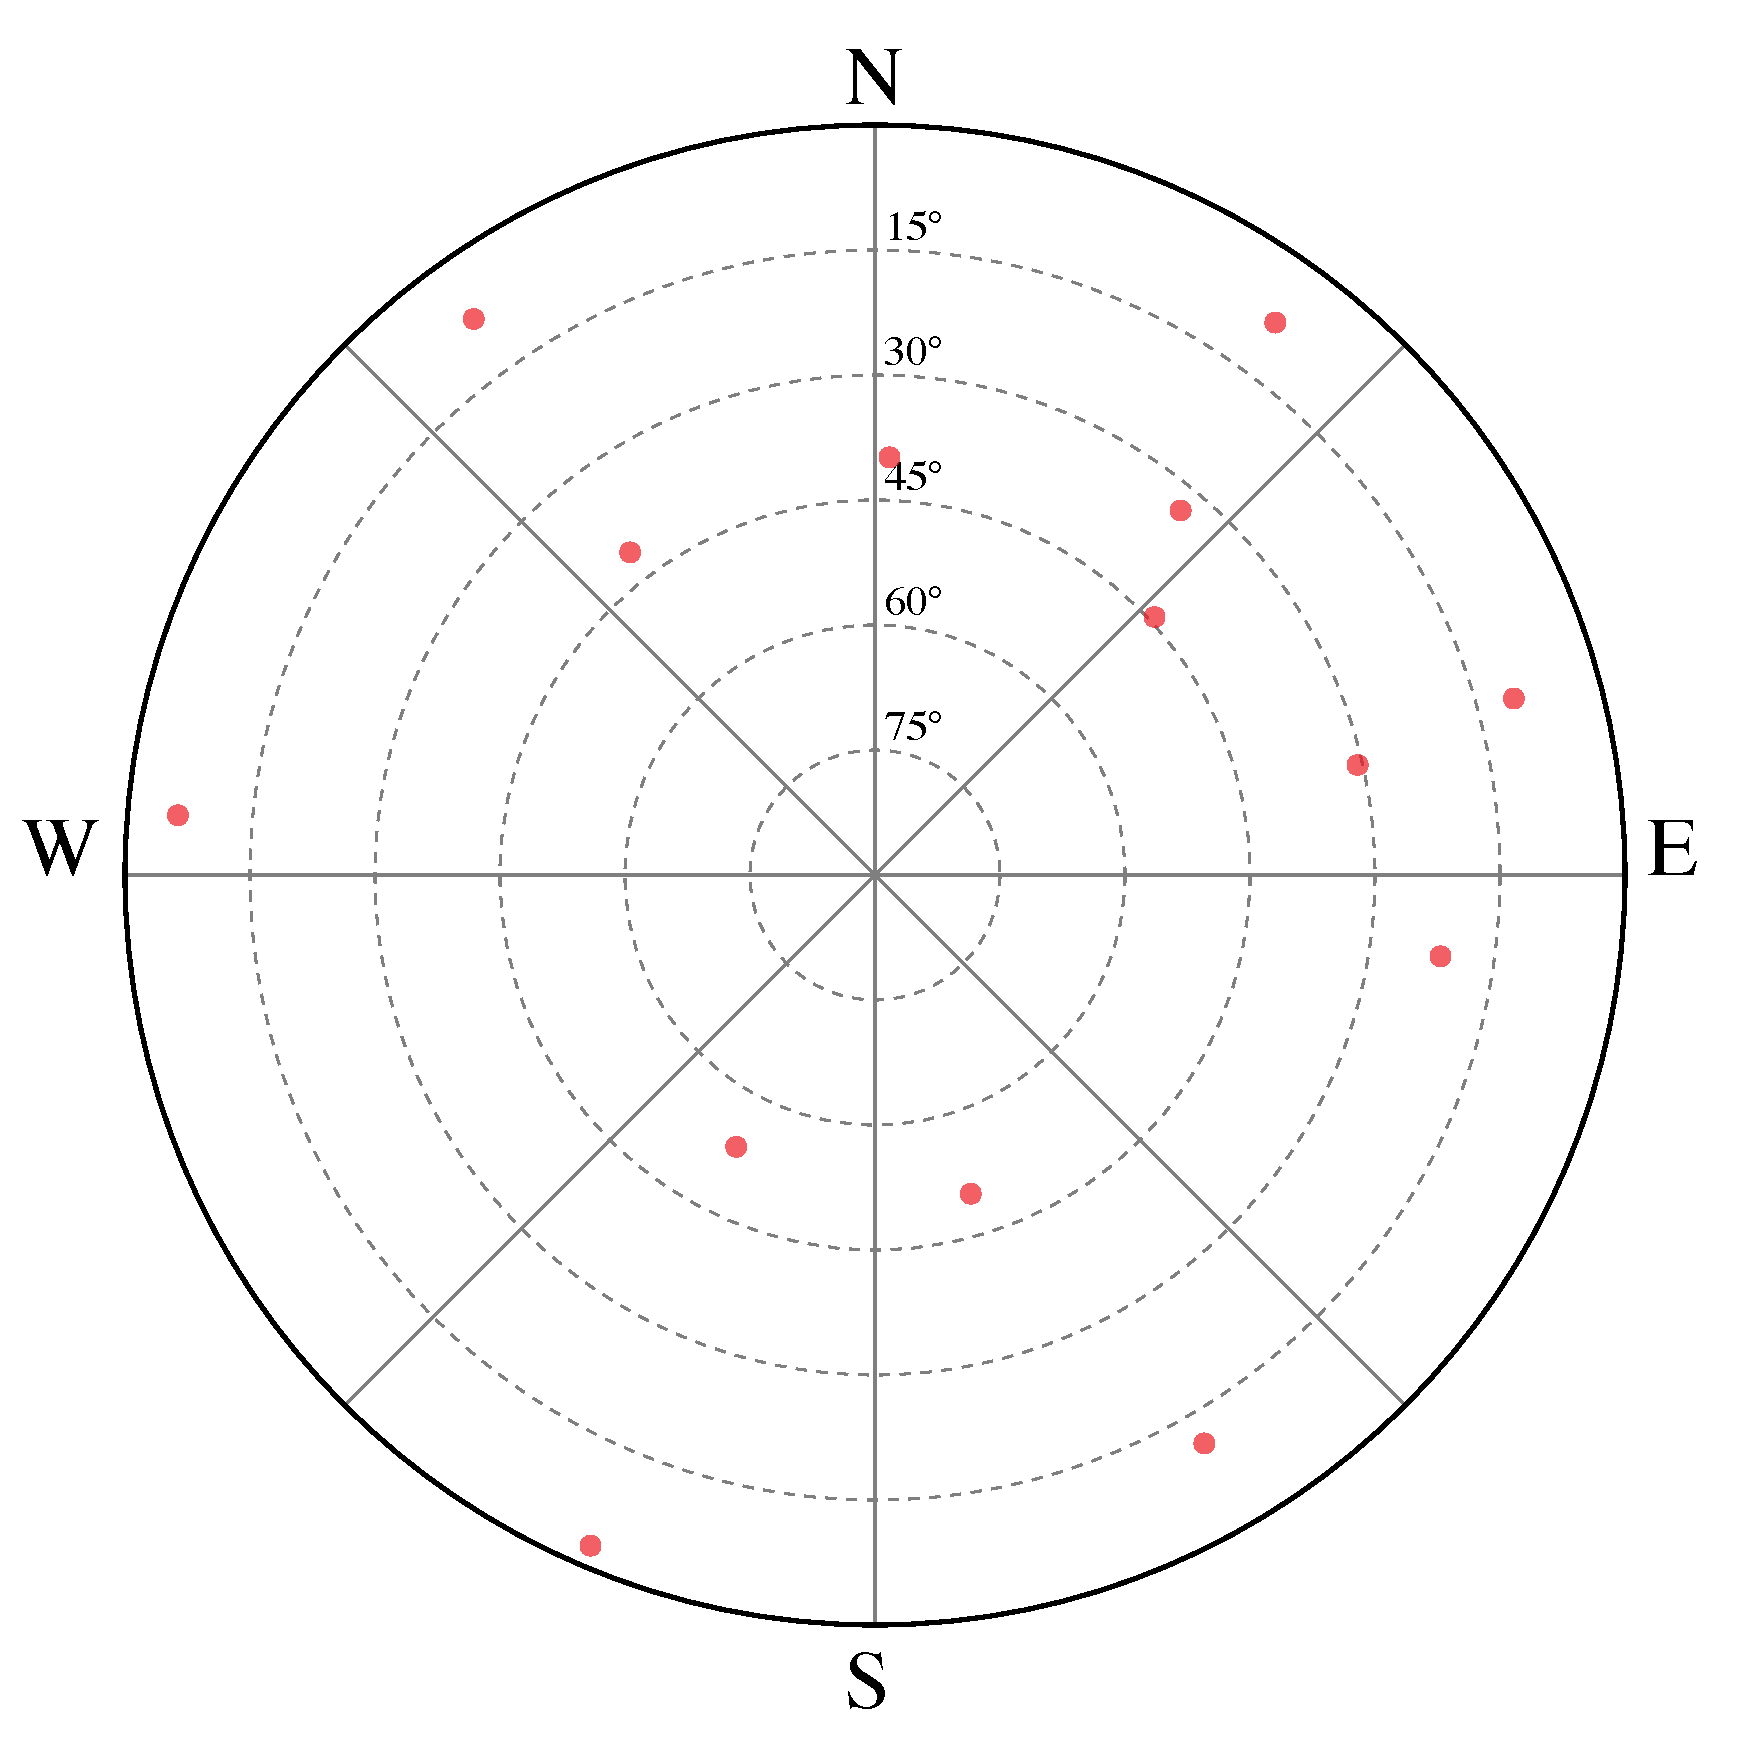
\includegraphics[width=1\textwidth]{Falcon9/Skyplot.pdf}
    \caption{}
    \label{fig:Skyplot}
\end{figure}



Space Exploration Technologies Corporation (SpaceX) is attempting to reduce launch costs by recovering the first stage of their Falcon 9-R launch vehicle. After first stage separation, the first stage performs a burn-back procedure, to fly back to the launch pad. During the burn-back, there is an inferred maximum de-acceleration of $\approx 7.8 g$ during the hypersonic burn, based on published performance figures. An overview of the flight profile can be found in figure \ref{fig:Falcon9Profile}. Additional information regarding the Falcon 9 V1.1 can be found in appendix \ref{ch:Falcon9}.

\begin{figure}[!htb] 
    \centering
    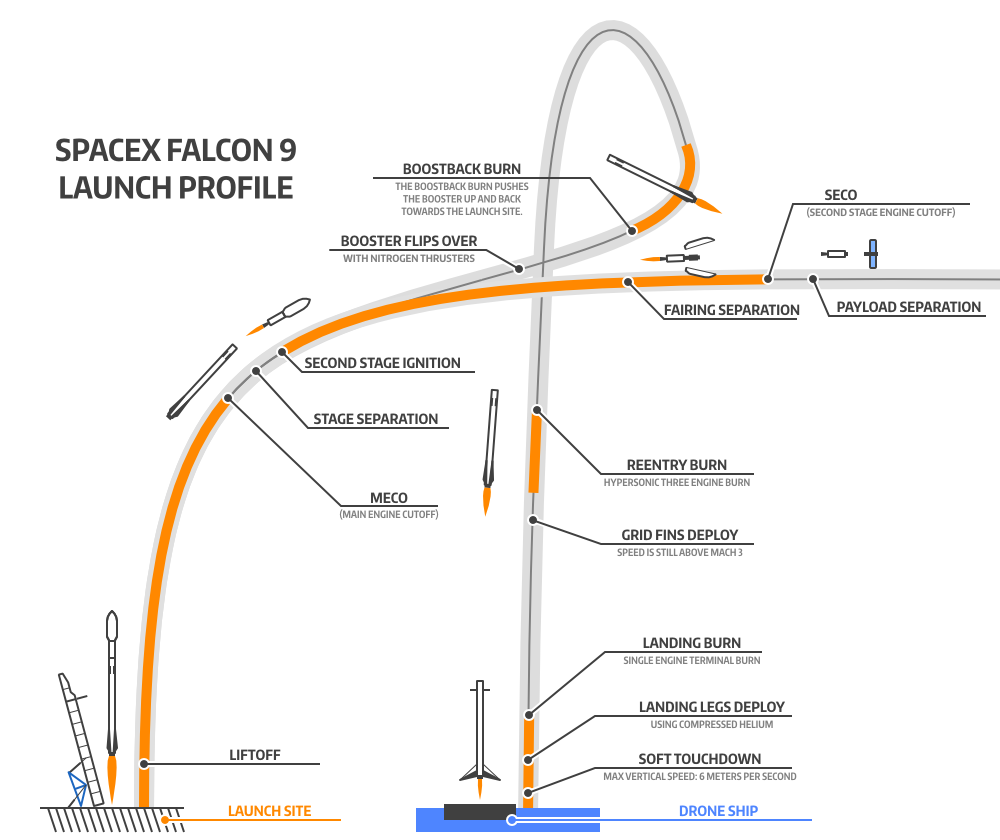
\includegraphics[width=1\textwidth]{FlightDynamics/Falcon9Profile.png} 
    \caption{An overview of the Falcon 9-R flight profile.}
    \label{fig:Falcon9Profile}
\end{figure}



